%
% Copyright (c) 2020 Antonio Coín Castro
%
% This work is licensed under a
% Creative Commons Attribution-ShareAlike 4.0 International License.
%
% You should have received a copy of the license along with this
% work. If not, see <http://creativecommons.org/licenses/by-sa/4.0/>.

Since the beginning of time, we humans have always had the need to store information of some kind for a variety of applications: to keep track of the grain stock, to make a census of the population of a certain area, or simply to make a note for latter use. But it was not until the start of the so-called \textit{era of information} that the storage of data in a digital format became a reality and a part of everyday life. From then on, there has been an ever-increasing need for storage capacity, growing from kilobytes to megabytes to gigabytes and beyond in a mere few decades. But in recent years, the quantity of data that we collectively manage has grown so large that it is even hard to comprehend its scale. To put things into perspective, the total estimate of data ever created, captured or replicated amounts to 18 zettabytes (more than $10^{13}$ gigabytes) \cite{rydning2018digitization}. That is indeed \textit{a lot} of data.

Given the enormous quantity of information that we are constantly generating, it should not come as a surprise that the conventional ways of storing, manipulating and analyzing this information fail to accomplish their goal: they have become outdated. This is why the search for new approaches to this problem has recently gained traction in industry as well as in academia; we require new architectures and methods for dealing with such a big volume of data. It is precisely for this reason that the term \textit{Big Data} was coined. It refers to the manipulation and the extracting of information from data sets so large that they exceed the capabilities of most modern operating systems and hardware, and cannot be handled with the usual data-processing methods within a reasonable elapsed time.

\section{Fundamental characteristics of Big Data}

First of all we need to clarify what we understand by Big Data. While the precise definition varies somewhat in the literature (see \cite{kitchin2016big} for example), there are a series of characteristics that any Big Data environment (problem, data set, etc.) should present in order for it to be considered as such. Coupled with these characteristics there are certain considerations to take into account, either as a direct result or as a side effect of working with large amounts of data. We explore all of these elements over the next subsections.

It should be noted that we will not consider a Big Data question the act of merely storing information with no other purpose than to preserve it. There should always be a particular problem (in the broad sense of the term) that is being solved by means of the data.

\subsection{The five V's}

The concept of the various \textit{V's of Big Data} has become a popular way of summarizing the principal characteristics that are desirable in a Big Data context. While the exact number and definition of these traits varies from author to author, they all share the same underlying principle: to capture the essence of what makes Big Data \textit{big}. We list below the ones that are deemed the most important, in no particular order.

\begin{enumerate}[1.]
  \item \textit{Volume}. It refers to the quantity of generated and stored data. It must be sufficient to draw meaningful conclusions and gain insight into the problem at hand. A necessary condition for establishing that some data has enough volume is that it exceeds the standard capacities of modern computers, which as of the year 2020 is in the terabytes.
  \item \textit{Velocity}. It relates to the speed or rate at which the data is generated or received. In some cases it includes real-time data processing, also known as \textit{streaming data}. In general, it is expected that the information be produced continually (think for example in a sensor of some kind).
  \item \textit{Variety}. The type and nature of the data also plays an important role. It includes both structured and unstructured data, drawn from various sources such as text, image, audio, etc.
  \item \textit{Veracity}. We can think of it as a way of measure how trustworthy the data is. The quality of the data can be affected by multiple factors such as inconsistencies, incompleteness or ambiguity, among others.
  \item \textit{Value}. It describes the added value that the collected data may have in the intended process, and the potential utility that can be extracted from the data. This value could change with time as the data is stored for a longer period, or even if the volume or velocity are modified.
\end{enumerate}


\subsection{Big Data algorithms}

Another relevant aspect apart from the above characteristics is \textit{how the data is being used}. In this work we focus on the analysis of said data to draw meaningful conclusions that could help solve a real-life problem. For this task the most common approach is to use the data to learn a specific pattern and try to generalize this behaviour to previously unseen data. This is essentially what is called a learning algorithm in the field of machine learning, in particular in \textit{supervised learning}. These algorithms are designed to solve a \textit{learning problem}, which in turn is almost always categorized as a \textit{classification problem} or a \textit{regression problem}.
In general, a learning problem can be formally stated as follows:

\begin{quotation}
  \itshape \noindent
  Let $X$ be an input space and $Y$ an output space, and suppose there is some kind of unknown relation between them, modelled by a function $f:X\to Y$. Further suppose that there is an underlying probability distribution $\mathcal P$ on $X \times Y$. The problem consists on estimating $f$ using a set of $n$ samples $\mathcal D = \{ (x_i, f(x_i)) \ | \ i = 1,\dots,n \}$ drawn independently and identically distributed from $X \times Y$ according to $\mathcal P$.
\end{quotation}
If the output space is discrete we say it is a classification problem (the elements of $Y$ are regarded as labels), and if it consists on a continuous range of values, we say it is a regression problem. One common example is analyzing medical data to extract information about a certain disease, or trying to predict if a patient will develop a condition based on some previously collected data from sensors, tests, etc.

Although the problem of learning from data was not born along with Big Data, it certainly has to adapt to this new setting. Often the well-known algorithms to solve tasks involving a controlled amount of data cannot be directly implemented to solve Big Data problems, and have to be redesigned with an essential feature in mind: \textit{scalability}. This property refers to the ability of algorithms to perform the task they were designed to do in a reasonable amount of time as the volume of data increases, if we equally increase the computation power of the machine where it is running. For example, an algorithm whose time complexity grows quadratically with the number of data points is not scalable, while one with a linear time complexity may very well be.

\subsection{Big Data ethics}

Since more and more data is being generated every day, there is a growing concern that this data could be used for malicious or unethical purposes. Of particular importance is the usage of \textit{personal data}, that is, data that could be used to identify a person or to extract information and patterns about their behaviour unbeknownst to them. In this regard there are a few principles that need to be taken into account when dealing with Big Data:

\begin{enumerate}[1.]
  \item \textit{Ownership}. This involves the rights over recorded data and the ability to exercise control over and limit the sharing of it. A recently passed European Union regulation called General Data Protection Regulation, or GDPR \cite{eu2016gdpr}, indicates that individuals own their personal data, and have a say in how it is being treated. This regulation clearly states that \textit{<<the processing of personal data should be designed to serve mankind>>}.
  \item \textit{Transaction transparency}. It refers to the right of any individual to have complete knowledge of why their data is being collected, how it is going to be used and for how long it will be stored, as well as how to amend any part of the collected data.
  \item \textit{Consent}. Before any use of personal data there must be an informed, explicit and unambiguous consent from the subject of the information.
  \item \textit{Privacy}. The idea that a reasonable effort should be made to preserve the privacy of the subjects of the data being collected is an important one. Anonymity should be guaranteed and under no circumstances should the data be used to or facilitate the task of identifying a particular person without their explicit consent and knowledge.
  \item \textit{Openness}. In an ideal setting, all data should be freely available and open to the general public. This is especially important when it comes to data gathered by governments, both for transparency and accountability reasons.
\end{enumerate}

\section{Big Data architectures}

Having reviewed the main properties and characteristics of Big Data, we conclude this introduction presenting the principal architectures and methods for the treatment of this data. There are roughly three areas in which the process can be divided: storage, processing and analysis.

We have already covered the analysis step, which consists on applying suitable algorithms to try to extract meaningful conclusions about the data, remembering that these algorithms must be developed in a scalable way. Not only should they be designed for scalability, but also adapted to be run on parallel architectures that allow the scalability to be implemented. In other words, in a Big Data environment it is typical to work with distributed machines, or \textit{clusters} of computers, so that more and more computing power can be easily added to the mix if needed.

Motivated by this approach arises the need for a method of storing data in multiple places in an efficient and safe way. Although there are multiple proposals to tackle this issue, one of the most prominent architectures is the \textit{Hadoop Distributed File System}\footnote{The name Hadoop comes from a toy elephant that belongs to the son of Doug Cutting, one of the main developers of the Apache Hadoop project.}, or HDFS \cite{chansler2010hdfs}. It provides an interface to store and access data in a distributed file system, and it is designed to be fault-tolerant and reliable.

As for the processing of the data, the reference framework is the MapReduce programming model, proposed by Google in 2004 \cite{dean2004mapreduce}. It consists on a \textit{mapping} stage, in which transformations are performed on the data, and a \textit{reduce} stage that serves as a summarizing or aggregating operation. These tasks are handled in a parallel fashion, and all communications and data transfers are managed by the framework.

As a final comment, we should point out that a trend that has emerged to facilitate dealing with these architectures is \textit{cloud computing}. Companies are offering their hardware resources for the public to rent and use as a way of working with Big Data, eliminating the need of physically assembling and maintaining a cluster of machines.

\subsection{Apache Spark}

Apache Spark\footnote{Full documentation available at \url{https://spark.apache.org/}.} is an open-source, distributed processing system and cluster-computing framework used to handle Big Data workloads in a fail-safe manner. It was released under its current name in 2014, and since then it has quickly become the \textit{de facto} standard for processing and analyzing large quantities of data. It has a large community of users who steadily make contributions and help improve and maintain the software. It also has a library specifically focused on distributed machine learning algorithms, called \textit{MLlib}, and some APIs specific to various programming languages, such as Python or Scala.

One of the main reasons for its popularity and acceptance is that under the hood Spark implements an improved version of the MapReduce architecture in a way that is transparent to the end user. This is achieved by utilizing a data structure known as \textit{Resilient Distributed Dataset}, or \acrshort{rdd} for short, which is an immutable distributed collection of objects. These datasets are stored in memory in a distributed fashion across many machines and can be manipulated via a series of transformations and actions to produce the desired result. As their name implies, there are a number of safeguarding mechanisms that prevent loss of data if a problem occurs in any of the datasets containers; they are designed to be fault-tolerant. One of the preventive measures taken is to keep track of the \textit{lineage} of each RDD, that is, the sequence of operations that were performed on it before it reached its current state, so that it can be reconstructed if needed.

With regard to the processing of the data, there is a \textit{master node} that controls all operations and is responsible for handing out pending tasks to the \textit{worker nodes} distributed across the cluster of machines. Sparks builds a directed acyclic graph (DAG) as a scheduling layer, which determines which tasks are executed on which nodes and in what sequence. In terms of the map-and-reduce model, the process is as follows:

\begin{enumerate}[1.]
  \item \textit{Map function}. The master node takes the input from the distributed file system or from memory, divides it into several sub-problems or \textit{partitions}, and transfers them to the worker nodes. Next, each worker node processes the data and performs transformations on it, transferring the result back to the master node. In every stage, data is stored and handled as a set of $\langle \text{key},\text{value}\rangle$ pairs.
  \item \textit{Reduce function}. The master node collects the answers of the worker nodes and combines them in a predefined way, acting on values that share the same key.
\end{enumerate}

It is worth pointing out that Spark implements a \textit{lazy evaluation} model consisting on \textit{transformations} and \textit{actions}. The so-called transformations are applied to an RDD and produce a new RDD. These transformation lazily stack together, without modifying any RDD in place, until an action is invoked on it. Then and only then the results are collected back to the main node, all the queued transformations are applied and the final action is performed. In this way, transformations are related to the mapping phase, while actions are linked to the reduce phase.

This platform requires a cluster manager and a distributed storage system to function properly. Popular choices regarding these components are Hadoop YARN and HDFS, respectively. We present below a review of the other principal components of the system and its workflow (see Figure \ref{fig:spark-workflow}), in Spark terminology:

\begin{itemize}
  \item \textit{Driver}. It is a separate process to execute user applications. It is responsible for scheduling jobs and negotiating with the cluster manager via its \textit{master node}.
  \item \textit{Node or Worker}. Any machine in the cluster that can run application code.
  \item \textit{Executor}. It is a process launched on a node, that runs tasks and keeps data in memory or disk storage.
   \item \textit{Task}. The minimal unit of work, executed by one executor on a single thread.
   \item \textit{Job}. A parallel computation that consists of multiple tasks that get spawned in response to an action.
\end{itemize}

\begin{figure}[h!]
  \centering
  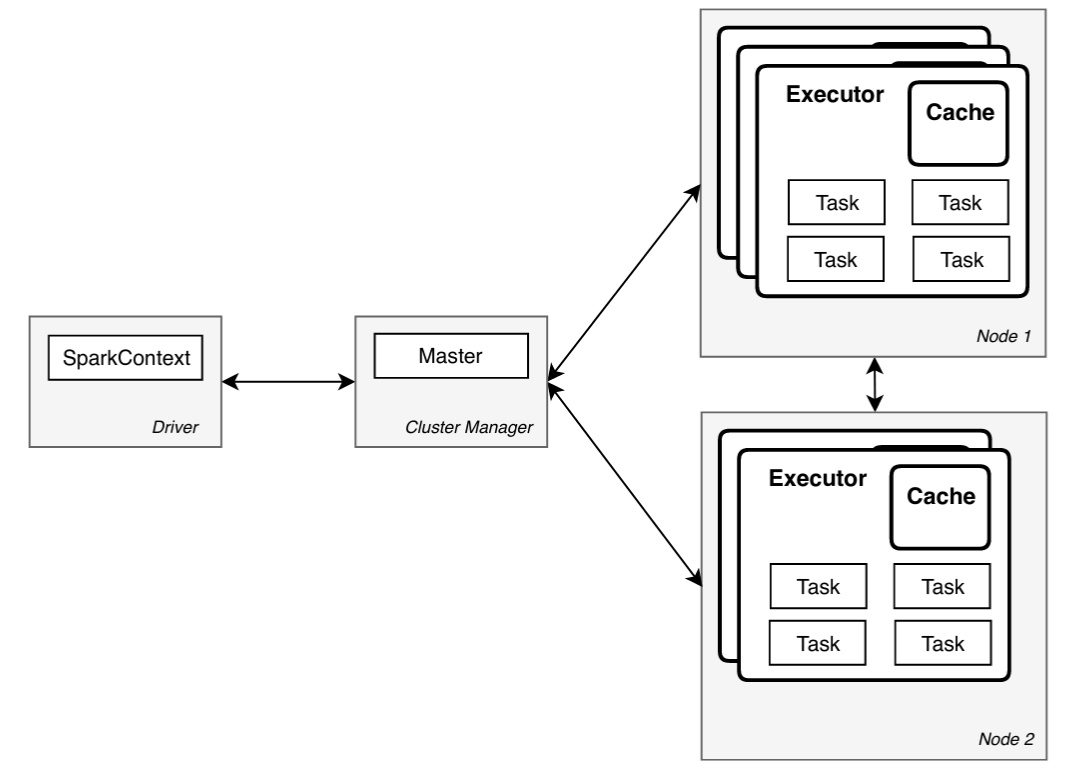
\includegraphics[width=.6\textwidth]{spark-workflow}
  \caption{Apache Spark components and schematic workflow. Taken from \cite{lopez2019distributed}.}
  \label{fig:spark-workflow}
\end{figure}
